\documentclass[11pt]{article}
\usepackage[pdftex]{graphicx}
\usepackage[margin=1in]{geometry}
\usepackage{fancyhdr}
\usepackage {abstract}
\renewcommand{\abstractname}{}   
\renewcommand{\absnamepos}{empty}
\usepackage{setspace}
\usepackage{svg}
\usepackage{float}
\usepackage{pythonhighlight}
\usepackage[most]{tcolorbox}
\setstretch{1.2}
\renewcommand{\sectionmark}[1]{\markright{\thesection.\ #1}} 
\renewcommand{\headrulewidth}{0.9pt}
\newcommand{\psettitle}[1]{
    \begin{center}
    \huge \textbf{#1}
    \end{center}
}

\abovecaptionskip

\newtcolorbox{examples}{
enhanced,
boxrule=0pt,frame hidden,
borderline west={4pt}{0pt}{colback=black!!white},
colback=white!10!white,
sharp corners
}


\title{Laboratory Report 1}								
\author{Linus C. Brendel}								
\date{\today}											

\makeatletter
\let\thetitle\@title
\let\theauthor\@author
\let\thedate\@date
\makeatother

\pagestyle{fancy}
\lhead{\textbf{Laboratory Report 1}}
\rhead{\textbf{\thepage}}
\cfoot{}
\setlength{\headheight}{1pt}

\begin{document}

\begin{titlepage}
	\centering
    \vspace*{0.5 cm}
    \includesvg[width=400pt]{logoNU.svg}\\[1.0 cm]	
    \textsc{\LARGE \textbf{Nazarbayev University}}\\[2.0 cm]
	\textsc{\Large \textbf{PHYS 161, PhLB 3}}\\[0.5 cm]							 
	\rule{\linewidth}{0.2 mm} \\[0.4 cm]
	{ \huge \bfseries \thetitle}\\
	\rule{\linewidth}{0.2 mm} \\[1.5 cm]
	
	\begin{minipage}{0.4\textwidth}
		\begin{flushleft} \large
			\textbf{{Student name:}}\\
			\textbf{1. Myrzakhan Yersultan}
            
                \textbf{2. Bakdaulet Shakirbay}
                
                \textbf{3. Galymzhan Baktybai}
			\end{flushleft}
			\end{minipage}~
			\begin{minipage}{0.4\textwidth}
			\begin{flushright} \large
            \vspace{-0.3cm}
			\textbf{Student Number:} \\
			\textbf{202338479}
            
            \textbf{202343094}
            
            \textbf{202343094}
		\end{flushright}
	\end{minipage}\\[2 cm]
	
	{\large{\textbf{Performance date: 30.12.25}}}\\[2 cm]
 
	\vfill
	
\end{titlepage}

\section*{Objectives:}

\begin{figure}[H]
    \centering
    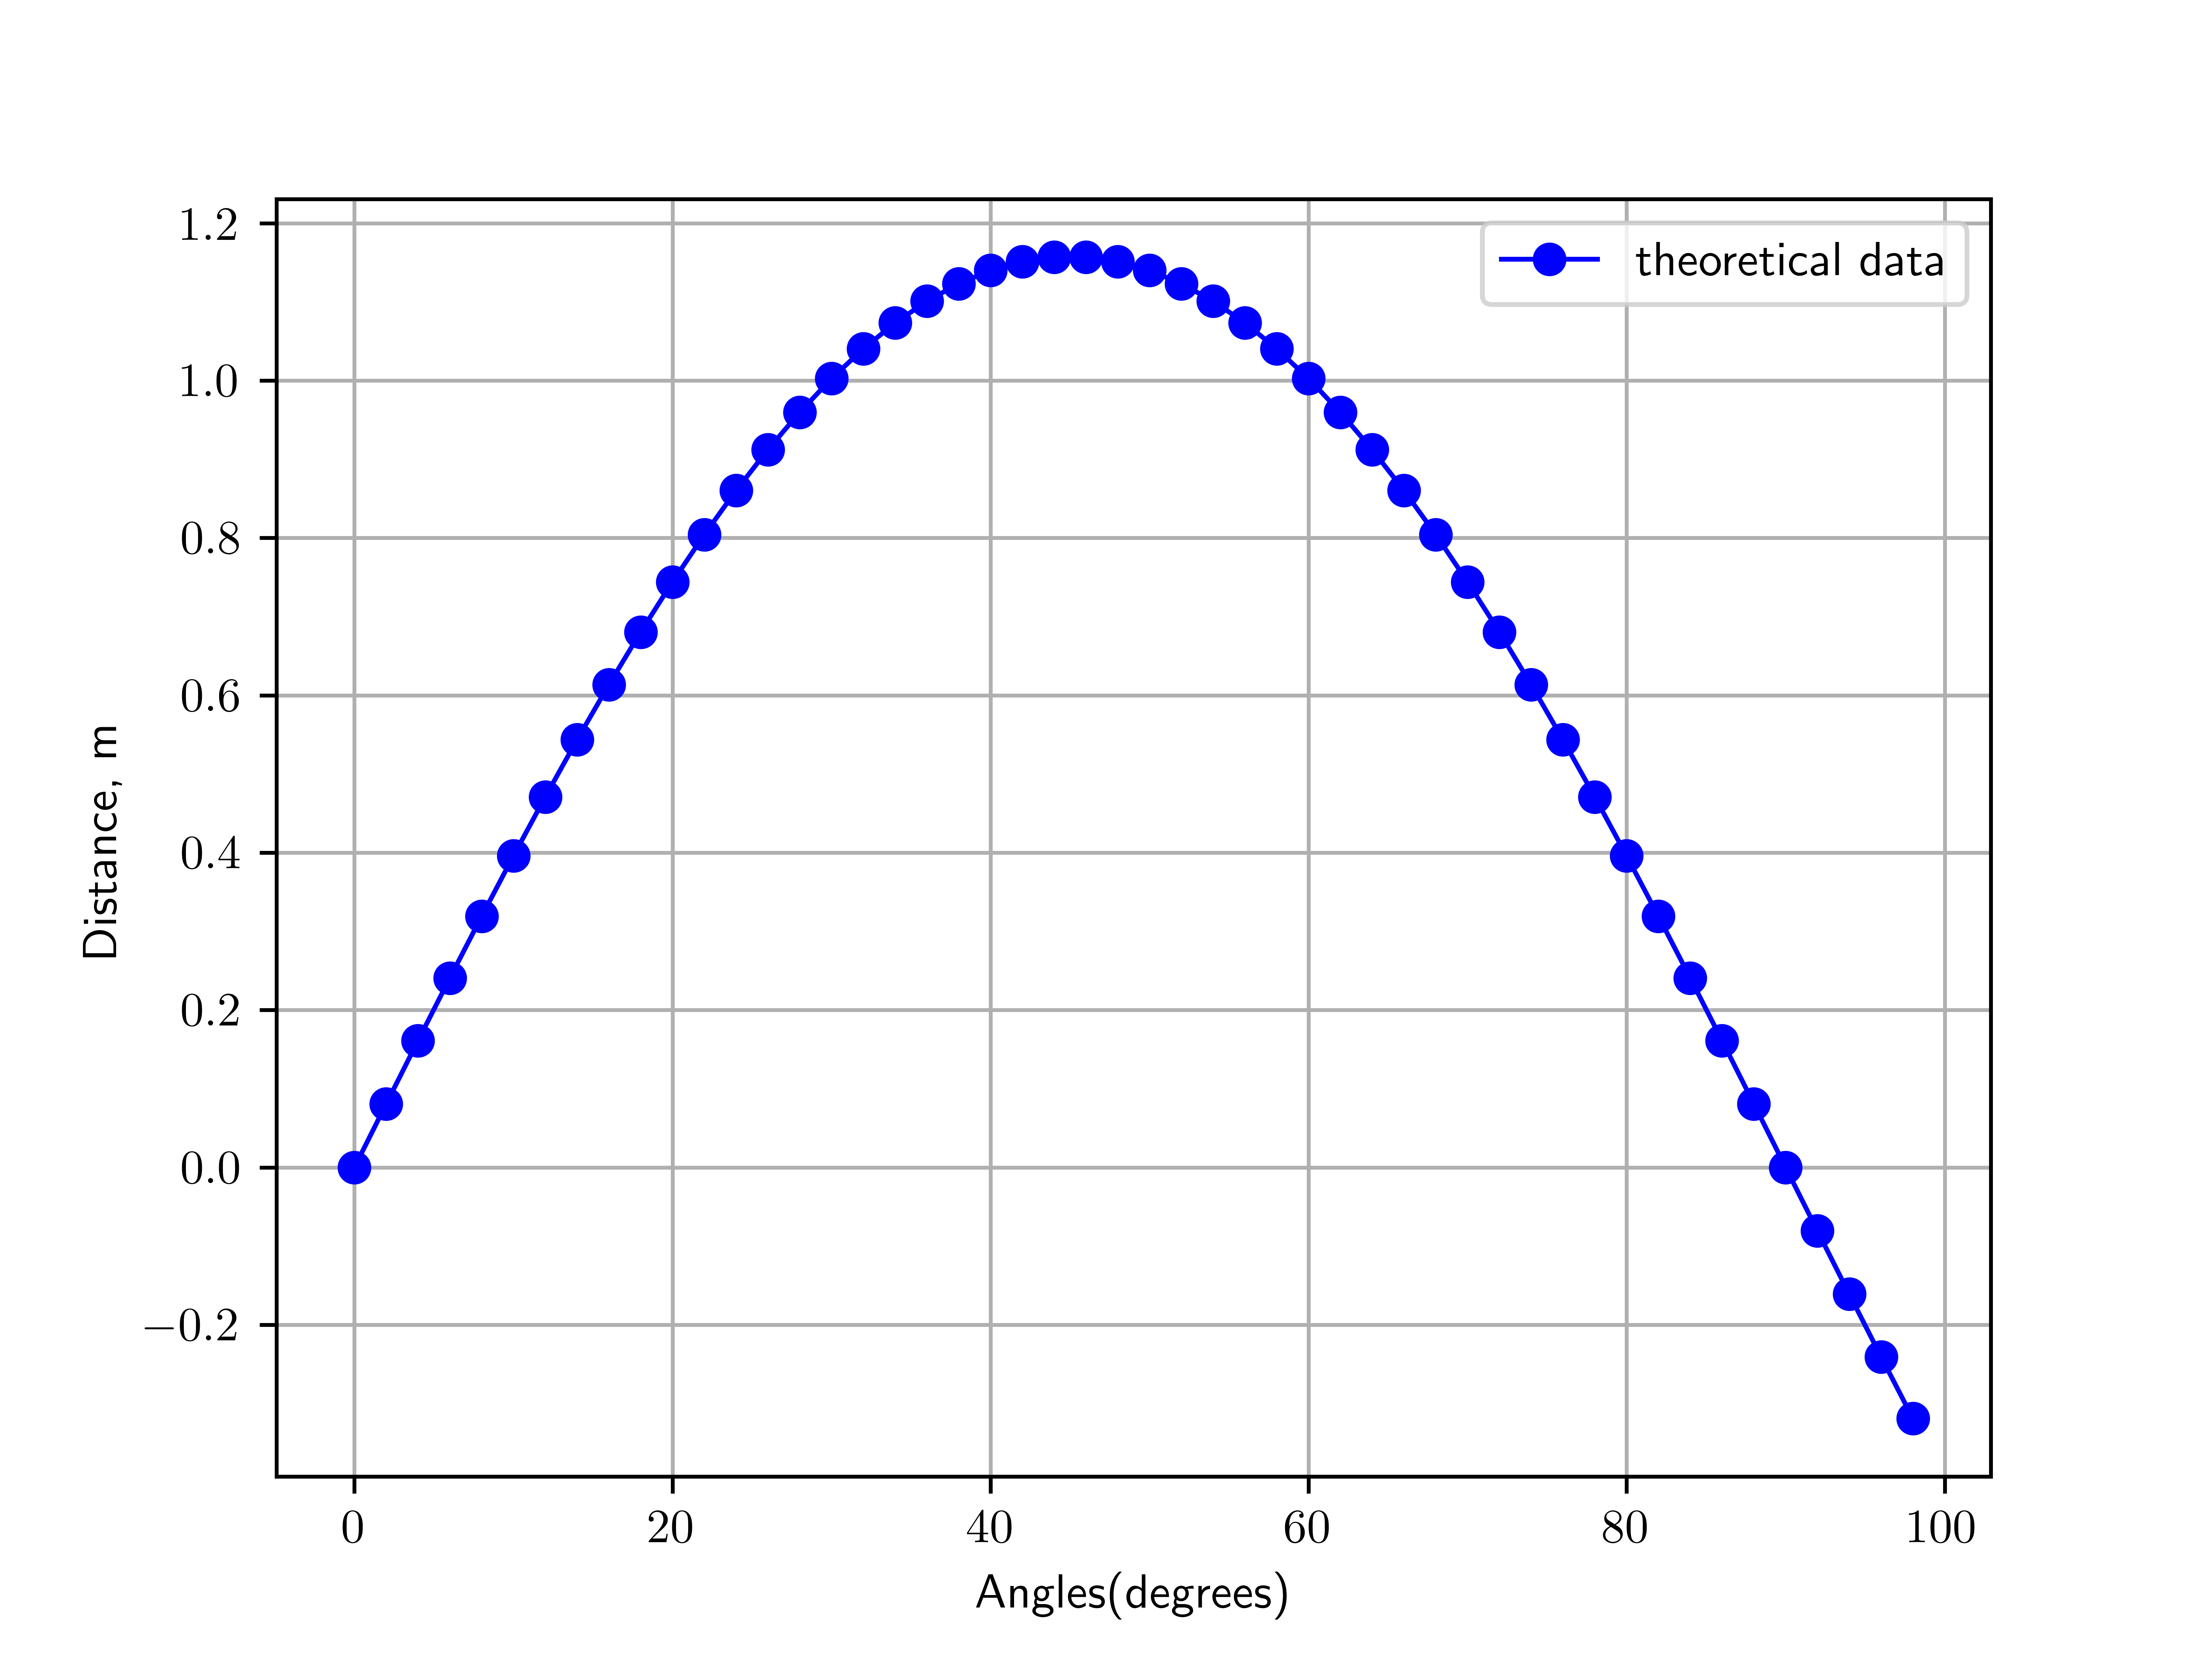
\includegraphics[width=1\linewidth]{rep.png}
    \caption{plot}
    \label{fig:erep}
\end{figure}

\begin{python}


import numpy as np
import matplotlib.pyplot as plt
import matplotlib as mlt
mlt.rcParams['text.usetex'] = True
from cycler import cycler

V=3.368
g=9.8
angles= np.arange(0, 100, 2)
def distance(angles):
    rad=np.radians(angles)
    return (2*V**2/g)*np.sin(rad)*np.cos(rad)

d=distance(angles)
with mlt.rc_context({'lines.linewidth': 1, 'lines.linestyle': '--', 'axes.prop_cycle':cycler(color=['blue'])}):
    fig, ax = plt.subplots()
    ax.plot(angles, d, 'b-o', label = 'theoretical data')
    ax.set(xlabel = 'Angles(degrees)', ylabel = 'Distance, m')
    ax.grid()
    plt.legend(loc='upper right')
    plt.savefig('rep.png', dpi = 1000)
    plt.show()
\end{python}



\end{document}